\documentclass{article}
\usepackage[utf8]{inputenc}
\usepackage{amsmath}

\title{Report on the Multi-User-MISO Simulation System Design}
\author{Zhan Zhang}
\date{October 2016}

\usepackage{graphicx}
\usepackage[margin=1.35in]{geometry}


\begin{document}

\maketitle

\section{Introduction}
Currently, the multi-antenna technologies have been widely used in the modern communication system standards.
Therefore building up software simulation platforms for multi-antenna communication systems have received much attention.
This report introduces the design of a simulation platform for
the multi-user-multi-input-single-output (MU-MISO) communication system.
Zero-forcing technology is applied for beam-forming and three different
power allocation algorithms are implemented. Performance evaluations are conducted based on the simulation platform.

\section{System Model}
\subsection{Overview}
In this simulation platform, the communication system transmits signals via \textit{J} transmission antennas to support \textit{K} users.
Each user is assigned with a single receive antenna. The scenario is modelled in Figure 1.
\begin{figure}[ht]
\centering
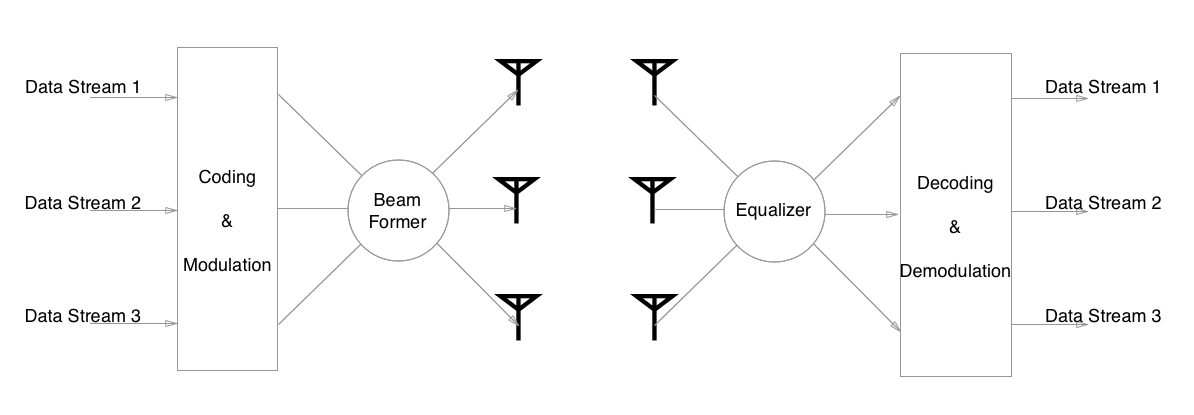
\includegraphics[scale=0.33]{Scenario.png}
\caption{The Scenario Model}
\label{fig:Scenario}
\end{figure}

\subsection{Channel Model}
The channel between the \textit{J} antennas and the \textit{k}th user is modelled as a column vector of length $\textit{J}$:
\[
\textbf{h}_k
=
\begin{bmatrix}
    h_{1k} \\
    h_{2k} \\
    \vdots\\
    h_{Jk}
\end{bmatrix} \hspace{1cm}(k = 1,...,K)
\]
where $h_{jk}$ stands for an i.i.d. random variable subject to $C\mathcal{N}(0,1)$ which represents the channel from the \textit{j}th
transmission antenna to the \textit{k}th user.

\noindent
The received signal for the \textit{k}th user could be derived as:
\[
\textbf{y}_k = \textbf{h}_k^H\textbf{x}+\textbf{n}_k \hspace{1cm}(k = 1,...,K)
\]
Where \textbf{x} is the beamformed sequence from the base station antennas,
$\textbf{n}_k$ is the additive white Gaussian noise (AWGN) for the $\textit{k}$th user,
and $\textbf{y}_k$ is the received signal for the $\textit{k}$th user.

\subsection{Zero-Forcing Beam Former}
The beam former is designed to eliminate the inter-user interference.
To match with all the \textit{J} antennas in the base station,
the beamformer for the \textit{k}th user would be modelled as a column vector:
\[
\textbf{w}_k
=
\begin{bmatrix}
    \textbf{w}_{1k} \\
    \textbf{w}_{2k} \\
    \vdots \\
    \textbf{w}_{Jk}
\end{bmatrix} \hspace{1cm}(k = 1,...,K)
\]
Thus the processed signal sequence \textbf{x} could be derived as:
\[
\textbf{x} = \sum_{k=1}^{K}\textbf{w}_k\textbf{s}_k
\]
The received signal $\textbf{y}_k$ becomes:
\[
\begin{split}
\textbf{y}_k = \textbf{h}_k^H\textbf{x}+\textbf{n}_k = \underbrace{
\textbf{h}_k^{H}p_1\textbf{w}_1\textbf{s}_1 +\textbf{h}_k^Hp_2\textbf{w}_2\textbf{s}_2
+\dots}_{interference}+\overbrace{\textbf{h}_k^Hp_k\textbf{w}_k\textbf{s}_k}^{signal}+
\underbrace{\dots+\textbf{h}_k^H\textbf{h}_Kp_K\textbf{s}_K}_{interference} +\underbrace{\textbf{n}_k}_{noise} \\
(k = 1,...,K)
\end{split}
\]
The zero-forcing beamformer is designed to eliminate the inter-user interference completely,i.e.,to make the interference part in the received signal equal to 0.
\[
\textit{interference} = \sum_{i = 1,i\neq k}^{K}\textbf{h}_k^H\textbf{w}_{i}\textbf{s}_{i} = 0
\]
As $\textbf{s}_{i}$ is the signal sequence of user \textit{k'}, $\textbf{s}_{k'} \neq 0$, the following condition needs to be fulfilled to cancel out the interference:
\[
\textbf{h}_k^H\textbf{w}_{i} = 0 \hspace{1cm}(i \neq k)
\]
From the pespective of the whole system serving \textit{K} users, the vectors of channels and beamformers could be merged into
two matrices \textbf{H} and \textbf{W}:
\[
\textbf{H}
=
\begin{bmatrix}
    \textbf{h}_{1} & \textbf{h}_{2} & \textbf{h}_{3} & \dots  & \textbf{h}_{K}
\end{bmatrix}
\]
\begin{center}
and
\end{center}
\[
\textbf{W}
=
\begin{bmatrix}
    \textbf{w}_{1} & \textbf{w}_{2} & \textbf{w}_{3} & \dots  & \textbf{w}_{K}
\end{bmatrix}
\]
To fulfill the requirement of the beamformer, the multiplication of matrices \textbf{H} and \textbf{W} should be equal to an identity matrix.
\[
\textbf{H}^H\textbf{W} = \textbf{I}
\]
where I is the identity matrix.

\noindent
Solving this equation, the zero-forcing beamformer \textbf{W} would be the pseudo-inverse of the channel matrix \textbf{H}:
\[
\textbf{W} = \textbf{H}^{\dagger}
\]

\subsection{Power Allocation}
The original beamformer would have a power gain larger than 1 which make the signal power exceeding the maximum output of the transmission antennas.
In this situation, we would allocate specific power gain to each user and rescale the beamformers according to the power allocation.

\noindent
The power allocated to the \textit{k}th user is denoted as $p_k$ and the power constraint of a transmission antenna is set to be P:
\[\sum_{k=1}^K p_k \leq P\]
and the power-allocated beamformer for the \textit{k}th user could be expressed as:
\[\textbf{w}_k = \frac{\textbf{w}_k\sqrt{p_k}}{\lVert \textbf{w}_k \rVert_{2}}\]
Three different power allocation methods are practiced in this system:
the Equal Receive Power Scaling Scheme, the Equal Transmit Power Scaling Scheme and the Water Filling Scheme.
\subsubsection{Equal Receive Power Scaling Scheme}
In the equal receive power scaling scheme, the initial beam former matrix is normalized by its Frobenius Norm:
\[
\textbf{W} = \frac{\textbf{W}}{\lVert \textbf{W} \rVert_{F}}
\]
The power allocated to the \textit{k}th user would be:
\[p_k = \frac{\lVert \textbf{w}_k \rVert_{2}^2}{\lVert \textbf{W} \rVert_{F}^2}\]
This normalization process would simply rescale the whole matrix with a constant to fulfill the limitation.
On the receivers' side, each user would be receiving same level of power under this scheme.

\subsubsection{Equal Transmit Power Scaling Scheme}
In the equal power scaling scheme, a uniform power is allocated to each user during transmission.
\[p_k = \frac{P}{K}\]
and the beamformer for each user become:
\[\textbf{w}_k = \frac{\textbf{w}_k\sqrt{P}}{\lVert \textbf{w}_k \rVert_{2}\sqrt{K}}\]

\subsubsection{Water Filling Scheme}
The water filling scheme is targeted to reach a maximum data rate for the whole group of users.
The method would allocate more power to those with better channel state to boost their achievable rate while meeting the power constraint.
Let the orignal beamformer gain to be $g_k$:
\[g_k = \lVert \textbf{w}_k \rVert_{2}^2\]
The maximum capacity problem could be expressed as:
\[
\max \sum_{k=1}^{K} log(1+p_k)
\]
with the limitation of
\[\sum_{k=1}^{K} p_k \leq P\]
Water filling method is efficient in solving this condition.
Set the water filling power to be $\mu$ and the maximization problem would be further transformed
to finding the maximum value of $\mu$ that satisfies:
\[\sum_{k=1}^{K}p_k \leq P\]
where the power allocated to the \textit{k}th user is:
\[p_k = (\mu-g_k)^+\]
 with $(x)^+$ denoting max\{x,0\} \cite{TY1}.

\noindent
Iterative half-division method is applied to find the value of $\mu$ to maximize the achievable rate.
An initial upper and a lower boundary are set for the $\mu$ and divided into two halves to locate the value of $\mu$ that would maximize the channel capacity.
At each iteration, the value of the upper boundary would be assume as the approximate value of $\mu$ and check whether it could meet the upper limit of the power constraint.

\noindent
The method would narrow the range of $\mu$ by half at each iteration and could achieve a satiable result after large number of iterations.
\subsection{Simulation Platform}
The system diagram for the simulation platform is shown in figure 2.
\begin{figure}[ht]
\centering
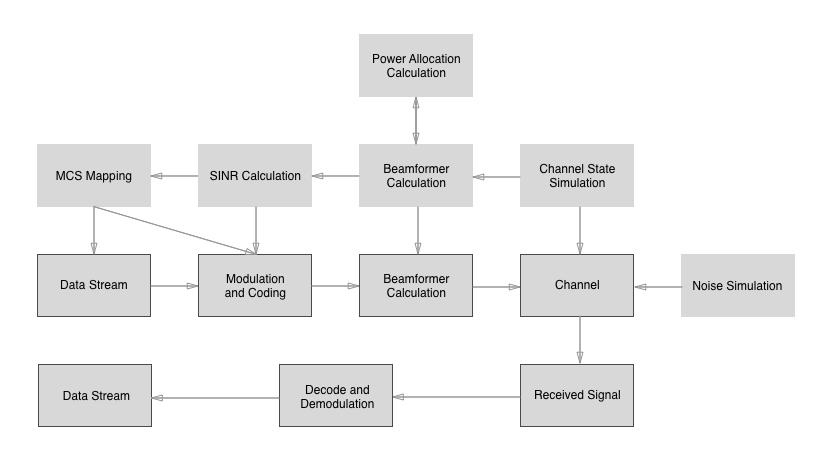
\includegraphics[scale=0.5]{SystemDia.png}
\caption{The System Diagram}
\label{fig:SystemDia}
\end{figure}

\noindent
The channel matrix \textbf{H} is firstly generated randomly and the corresponding beamformer \textbf{W} is calculated.
Additive white Gaussian noise is generated as a random vector $\textbf{n}_k$ for the \textit{k}th user with the noise power $\sigma^2_k$.
A data stream of a block length is simulated for each user for transmission.
Signal-to-Interference-and-Noise-Ratio for each user is then calculated to determine the modulation and coding scheme.
The SINR for the \textit{k}th user is:
\[
SINR_k = \frac{P_{Signal}}{P_{Interference}+P_{Noise}} = \frac{\textbf{h}_k^H\textbf{w}_k\textbf{w}_k^H\textbf{h}_k}{\sum_{i = 1,i\neq k}^{i = K}\textbf{h}_k^H\textbf{w}_i\textbf{w}_i^H\textbf{h}_k+\sigma_k^2}
\]
where the $\textbf{w}_k$ is the beamformer for the \textit{k}th user with the power component multiplied.

\noindent
The SINR is converted into decimal scale and mapped to the corresponding CQI and MCS index values.
$$SINR(dB)_k = 10*log_{10}(SINR_k)$$
With the specific modulation and coding scheme, a data stream of a block length is randomly generated for each user.
All the data streams are converted into the signal sequences \textbf{s}
and \textbf{s} for all users then pass through the beamformer and form the signal \textbf{x}.

\noindent
Beamformed signal \textbf{x} would be simulated-transmitted via the channel and reach the user.
The user side would decode, demodulate and detect the received signal.

\noindent
The decoded data stream at the user side would be directly compared to the original one for evaluation.


\section{Performance Evaluation and Comparison}
The detected data streams are compared to the original ones and check if there is any error. The blocks successfully transmitted are counted to the total throughput.
\[ThroughPut_k = L_{Bl}N_{Bl}\]
where $L_{Bl}$ is the block length of the specific modulation and coding scheme and the $N_{Bl}$ is the number of blocks which are transmitted correctly.

\noindent
The achievable rate for the \textit{k}th user is calculated from the SINR values:
$$AcRate_k = FB_wlog_2(1+SINR_k)$$
where F denotes the system loss of the OFDM system, and $B_w$ stands for the bandwidth of the channel.

\noindent
The comparison between the total throughput and the total achievable rate for all users is conducted to evaluate the performance.
The performance of the system applying the two power allocation schemes is shown in figure 3 (2-user-2-input-single-output system).


\begin{figure}[ht]
\centering
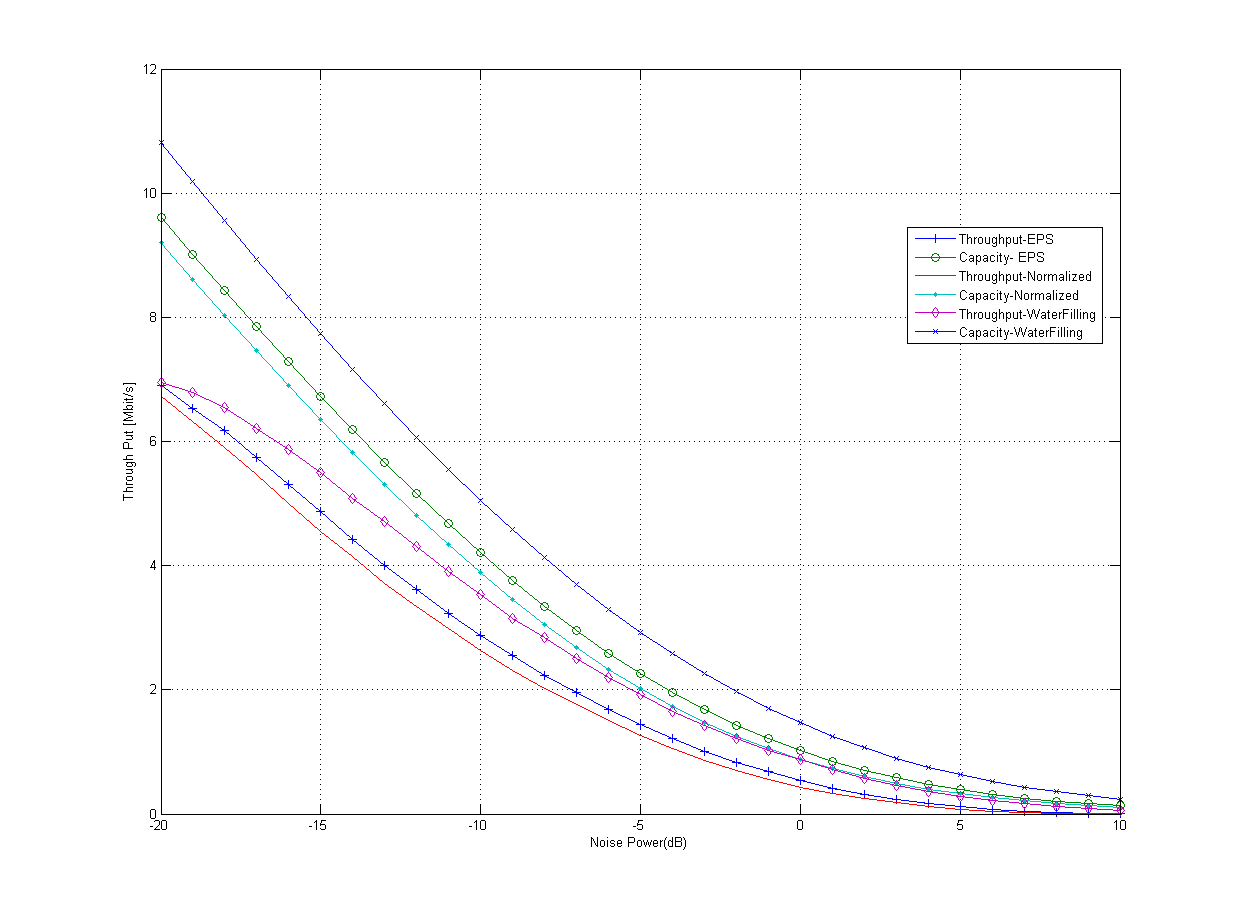
\includegraphics[scale=0.45]{Comparison.png}
\caption{Comparison Between the 3 Power Allocation Methods with Zero-Forcing MU-MISO System}
\label{fig:Comparison}
\end{figure}

\noindent
The waterfilling power allocation method performs better in the total throughput comparing to the other two algorithms.
However, the increase in total throughput is traded with the loss of throughput for users with poor channel state.

\noindent
The equal transmit power scaling method outstands in equality for all user and has a relatively good performance comparing to the normalized method.
When the channel for all users is quite good, the performance of both the equal power scaling and waterfilling scheme would become quite similar.

\noindent
The equal receive power scaling method would be the simplest in implementation. However, this advantage over the equal power scaling scheme is nearly ignorable.

\noindent
The performance of the adaptive Single-Input-Single-Output(SISO) system is shown in figure 4. Comparing figure 3 and figure 4,
 performance is much boosted for the zero-forcing MU-MISO system comparing to the SISO system with both power allocation schemes.
\begin{figure}[ht]
\centering
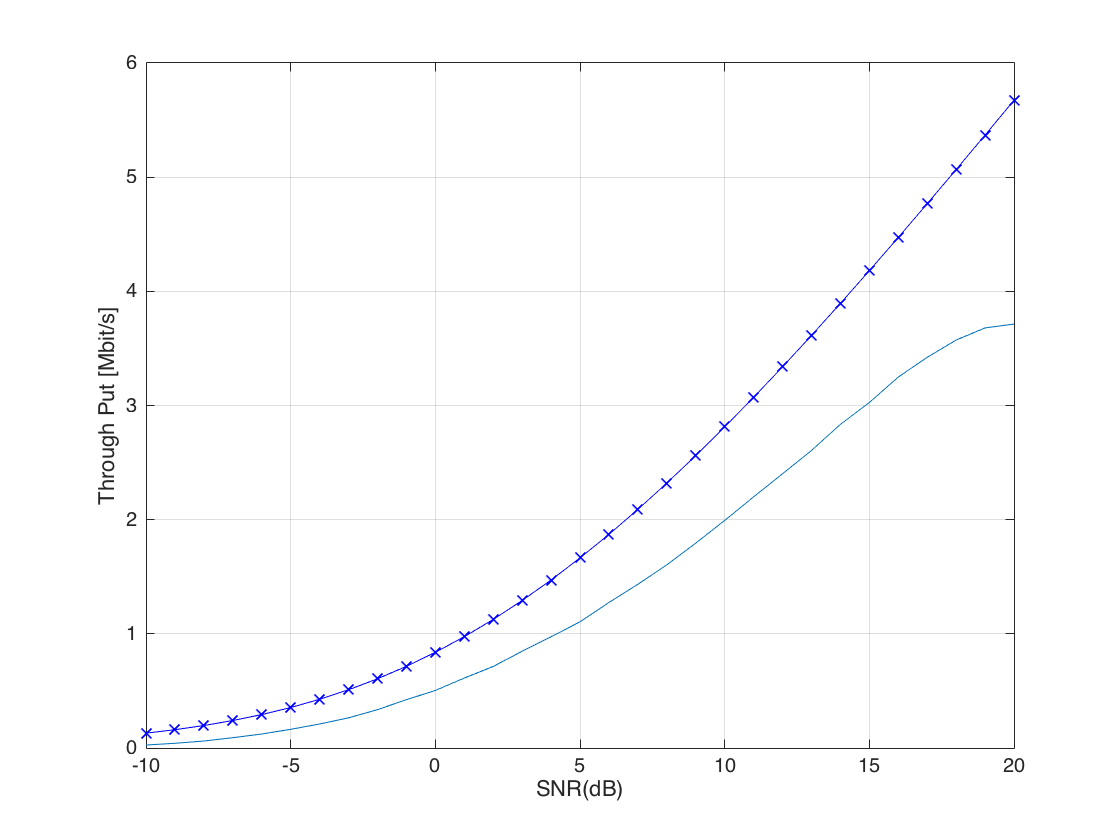
\includegraphics[scale=0.4]{FadingSISO.png}
\caption{SISO Performance}
\label{fig:SISO}
\end{figure}


\section{Conclusion}
The simulated Multi-User MISO system with Zero-Forcing beamforming performs far better in term of total throughput. Therefore it would be
more suitable for the multi-user scenario, which becomes more and more common in the modern world.
The multi-antenna technology would be replacing the SISO system in modern communication systems to achieve better performances for
real-world multi-user scenarios.

\noindent
The water filling algorithm outstands in term of total throughput but fails to keep quality for users with poor channel state.
The equal transmit power scaling method would work well in good channel state and keep equality to all users when channel becomes poor.
The equal receive power scaling method has a relatively poor performance comparing to the other two. The advantage in the simplicity is also small thus is not widely used in practice.

\bibliographystyle{plain}
\bibliography{references}{}
\end{document}
